% --------------------------------------------------------------------

\section{Johdanto}

Ohjelmistoprojekteissa tulee väistämättä vastaan ongelmia. Näiden järjestelmällinen analysointi ja ehkäiseminen jatkuvana osana kehitysprosessia parantaa ohjelmistoprojektin mahdollisuuksia onnistua. Ketterässä ohjelmistokehityksessä kehitystiimi järjestää säännöllisesti reflektion, jossa tiimi tarkastelee työtapojaan ja tiimityöskentelyään, sekä pohtii tapoja, joilla voi sopeuttaa niitä päästäkseen parempiin tuloksiin \citep{AgileRetros2006}. Tiimi pyrkii tutkimaan konkreettisia ongelmia ja löytämään niihin konkreettisia ratkaisuja \citep{AgileRetros2006}. Juurisyyanalyysi tarjoaa rakenteellisen tavan löytää ongelmien aiheuttajia ja voi siten auttaa ehkäisemään näiden ongelmien esiintymistä jatkossa \citep{Lehtinen2011}. Siksi se sopii hyvin käytettäväksi ongelmanratkaisumenetelmäksi retrospektiiveihin (tähän viite esim ESEM paperiin). Juurisyyanalyysiä voi kuitenkin tehdä lukuisalla eri tavalla \citep{Lehtinen2011}.

Vaikka iteraation lopussa pidettävä retrospektiivi on olennainen osa ketterän ohjelmistokehitysprosessin runkoa, ei sen toteutustapavasta ole yhteistä käytäntöä. Retrospektiivin järjestäminen on määritelty ketterien menetelmien yleisissä periaatteissa \citep{AgileManifestoPrinciples}. Retrospektiivin tavoitteet saattavat olla määritelty tarkasti metodologian kuvauksessa, mutta sen toteutustapa on usein jätetty yleensä tiimin päätettäväksi. Esimerkiksi Scrum-metodologian kuvauksessa on kuvattu retrospektiivien tavoitteet, muttei niiden saavuttamiseen johtavia menetelmiä \citep{ScrumGuide2011}.

Tässä kandidaatintyössä tutkitaan systemaattisen kirjallisuuskatsauksen \citep{Kitchenham2010} muodossa, minkälaisia menetelmiä aiemmassa kirjallisuudessa on esitetty juurisyyanalyysiä soveltaviin retrospektiiveihin. Työssä pohditaan myös, minkälainen menetelmä voisi sopia ketterän ohjelmistokehitystiimin retrospektiiviin.  Menetelmän tulee olla erittäin kevyt ja yksinkertainen, jotta sen käyttöönotto lyhyehköissä iteraatio-retrospektiiveissä olisi mielekästä. Esimerkiksi extreme programming -metodologiaan on suositeltu lyhyitä ja tehokkaita retrospektiivejä, jotka eivät vaadi kovin suurta panosta tiimiltä, mutta tuottavat siitä huolimatta välittömiä ja näkyviä tuloksia \citep{myllyaho2004review}.

Kandidaatintyön työmäärän pitämiseksi järkevänä, on systemsaattisessa kirjallisuuskatsauksessa käsiteltävän kirjallisuuden joukkoa rajattu eri tavoin. Aineistohaut rajoitetaan Scopus-tietokannan tieteellisiin artikkeleihin. Käytettävät hakusanat on määritelty yhdessä kandidaatintyön ohjaajan kanssa. Muut rajaukset esitellään kandidaatintyön menetelmät-osiossa.

Tämä kandidaatintyö on jaettu seuraaviin osiin. Kappaleessa 2 esitellään teoreettinen tausta, eli esitellään ja määrittellään kirjallisuuden avulla termit "ketterä retrospektiivi" ja "juurisyyanalyysi". Tämän jälkeen kuvataan työssä käytetty systemaatinen kirjallisuuskatsaus menetelmä. Kappaleessa 4 tuodaan julki tulokset ja kappaleessa 5 tulosten johtopäätösket. Kandidaatintyön viimeinen kappale on yhteenveto.

\section{Teoreettinen tausta}
\subsection{Ketterä retrospektiivi}
Ketterissä ohjelmistokehitysmenetelmissä on määritelty, että säännöllisin väliajoin pidetään reflektointi, jossa tiimi pohtii tapoja tulla tehokkaammaksi. Nämä kehitettyjen parannusten perusteella tiimi muuttaa toimintaansa \citep{AgileManifestoPrinciples}. Kevyt retrospektiivisessio on tapa toteuttaa tätä periaatetta. Projektin lopputuloksen kannalta retrospektiivejä on järkevää pitää lyhyin väliajoin. Tällöin tiimin kohtaamat ongelmat ja niihin liittyvät yksityiskohdat ovat tuoreessa muistissa ja parannusehdotukset voidaan ottaa suoraan käyttöön ja siten pyrkiä parantamaan projektin lopputuloksen laatua. \citep{Cockburn2002}

XP- ja Scrum-metodologiassa retrospektiivejä suositellaan pidettäväksi joka iteraation päätteeks. Niissä tiimi reflektoi sitä, missä he ovat viime iteraation aikana onnistuneet hyvin ja missä on vielä kehitettävää. \citep{Lindstrom2004, ScrumGuide2011} Retrospektiivin avulla tiimi saa palautetta työstään. Retrossa voidaan muun muassa pohtia sitä, miten kurinalaisesti tiimi on noudattanut seuraamansa metodologian käytäntöjä ja voisiko niitä räätälöidä sopimaan paremmin tiimin tarpeisiin. \citep{Lindstrom2004}

\subsection{Juurisyyanalyysi}
Juurisyyanalyysi on rakenteellinen tapa tutkia ongelmia ja tunnistaa niiden aiheuttajia. Ideana on se, että korjaamalla syyn aiheuttavia ongelmia voidaan ehkäistä saman ongelman syntymistä uudestaan -- tai ainakin vähentää ongelman uudelleenesiintymisen todennäköisyyttä. \citep{Lehtinen2011} Juurisyyanalyysin avulla voidaan tutkia ongelmien lisäksi myös onnistumisten syitä. \citep{Bjornson2009} Juurisyylle on useita määritelmiä. Se voi tarkoittaa mitä tahansa ongelman aiheuttavaa syytä, syyketjun perimmäisintä syytä tai syytä, johon johtoporras voi vaikuttaa. Juurisyyanalyysin tuloksia voidaan käyttää apuna prosessinkehityksessä. \citep{Lehtinen2011}

\section{Systemaattinen kirjallisuuskatsaus tutkimusmenetelmänä}


kamaa johdannosta, katso sopiiko tänne:\\
\textit{Käytettävät hakusanat, joita haetaan artikkelien otsikosta ja avainsanoista, ovat "retrospective", "postmortem analysis", "post-project review" ja "software engineering". Artikkelien tulee olla julkaistu aikaisintaan vuonna 1990. Mikäli näillä rajauksilla löytyy liikaa artikkeleita, tarkennetaan hakua. Liian rajaavien termien, kuten "root cause analysis" tai "agile", käyttöä pyritään kuitenkin välttämään. Näitä käyttämällä saattaisi ohittaa kiinnostavia artikkeleita, jotka käsittelevät olennaisia asioita, mutta eri termejä käyttäen. Eri hakusanayhdistelmillä löytyneiden tulosten määrä kirjataan ylös.
Hakutuloksista olennaisia ovat sellaiset, jotka kuvaavat jonkinlaista menetelmää käytettäväksi retrospektiiveihin. Nämä artikkelit kerätään taulukkolaskentaohjelman viitekokoelmaan, jossa ylläpidetään artikkeleista kaikkia lähdeviitteeseen tarvittavia tietoja, sekä merkinnän siitä, onko artikkelissa kuvattu retrospektiivin menetelmä juurisyyanalyysi. Ne artikkelit, jossa menetelmä sisältää juurisyyanalyysin, päätyvät kandidaatin työhön. Systemaattisen kirjallisuustutkimuksen tarkoituksena on tehdä aineistonhakuprosessista tarkastettava ja toistettava \citep{Kitchenham2007}.}




\subsection{Taustaa}
Systemaattisessa kirjallisuuskatsauksessa (SLR, Systematic Literature Review) tehdään kattava arviointi valitusta aiheesta. Arvioinnissa käytetään luotettavaa, tarkkaa ja toistettavisaa olevaa menetelmää. SLR on kirjallisuuskatsauksen muoto, mikä tarkoittaa sitä, että siinä käydään läpi aiempia tutkimuksia, jotka ovat olennaisia omien tutkimuskysymysten valossa. Kerätyn kirjallisuuden pohjalta muodostetaan synteesi.\citep{Kitchenham2007}

SLR:n erityispiirteenä on se, että kirjallisuuden etsiminen, valikointi ja valitun kirjallisuuden analysointi pyritään tekemään toistettavasti ja puolueettomasti. Kitchenham perustelee SLR-menetelmän hyötyä toteamalla, että kirjallisuuskatsaus, joka ei ole SLR:n tapaan perusteellinen ja tasapuolinen ei tarjoa paljoa tieteellistä arvoa. Systemaattisen kirjallisuuskatsauksen tulokset ovat todennäköisemmin puolueettomia, eli tutkijan kannasta riippumattomia. \citep{Kitchenham2007}

Systemaattinen kirjallisuuskatsaus koostuu kolmesta päävaiheesta: suunnittelu-, toteutus- ja raportointivaiheista. Suunnitteluvaiheessa tunnistetaan kirjallisuuskatsauksen tarve, määritellään tutkimuskysymykset, sekä protokolla katsauksen suorittamiselle. \citep{Kitchenham2007}

Toteutusvaiheessa tehdään aineistohakuja ja valitaan ennaltamääritellyin kriteerein tutkimukselle olennaiset artikkelit. Artikkelien laatua ja sitä kautta luotettavuutta arvioidaan. Tehdyistä hauista kirjataan kaikki kirjallisuuskatsauksen toistamiseen ja sen laadun arviointiin tarvittava tieto, kuten haussa käytetyt hakukoneet, hakusanat, löydettyjen tulosten määrä ja jopa tuloslista. Valitusta aineistosta kerätään tietoa talteen ja sen merkittävyyttä omalle tutkimukselle arvioidaan ennalta määritellyin kriteerein. Kerätyn ja merkittäväksi valitun tiedon perusteella muodostetaan synteesi. Raportointivaiheessa kirjoitetaan tulokset ylös ja arvioidaan tuloksia. \citep{Kitchenham2007}

Tähän kandidaatintyöhön valittiin Kitchenhamin määrittelemä systemaattinen kirjallisuuskatsaus, jotta kerätty aineistolista ja sen pohjalta saadut tulokset olisivat tieteellisesti merkittävämpiä, sekä mahdollisesti myös muulle tutkimukselle käyttökelpoisia.

\subsection{Rajaukset}
Ennen kirjallisuuskatsauksen aloittamista kandidaatintyön ohjaajan kanssa sovittiin seuraavat rajaukset. Aineistohaut suoritettaisiin pelkästään Scopus-tietokantaan. Haku rajataan pelkkiin tieteellisiin artikkeleihin. Haetut artikkelit eivät saa olla julkaistu ennen vuotta 1990. Myös käytettävät hakusanat sovittiin alustavati kattamaan sanat "retrospective",  "postmortem analysis", "post-project review" ja "software engineering". Näistä hakusanoista tulisi kokeilla erilaisia yhdistelmiä.

Rajaukset tehtiin, jotta kandidaatintyön työmäärä pysyisi järkevänä. Seuraavaksi käydään läpi yksittäisten rajausten perustelut. Scopus-tietokanta valittiin kandidaatintyön ohjaajan suosituksesta. Haku rajattiin tieteelliset artikkelit valittiin, koska ne tieteellisten julkaisujen tiukasta artikkelien karsintaprosessista johtuen todennäköisimmin sisältäisivät tieteellisesti merkittävää tietoa. Vuosi 1990 valittiin, koska niihin aikoihin julkaistiin ensimmäiset artikkelit juurisyyanalyysistä (tähän viite). Hakusanat valitiin sisältämään eri nimityksiä retrospektiiveille, joita on retrospektiivin lisäksi muun muassa "post-mortem analysis" ja "post project review". Nämä ovat yleensä projektitasolla järjestettyjä retrospektiivejä. Ohjelmistotuotanto ("software engineering") valittiin hakusanaksi rajaamaan haku kattamaan ainoastaan ohjelmistotuotannon alan retrospektiivit.

Ajatuksena oli tehdä haku retrospektiivin näkökulmasta ja löytää sieltä viitteitä juurisyyanalyysin käytöstä. Kirjallisuuskatsauksessa olisi siis tarkoituksena hakea retrospektiiveihin liittyviä artikkeleita, löytämään niistä retrospektiiveihin käytetty menetelmä ja tarkistamaan, sisältääkö kuvattu menetelmä juurisyyanalyysin.

\subsection{Hakutermin muodostuminen}
Kandidaatintyön kirjoittaja aloitti systemaattisen kirjallisuuskatsauksen kokeilemalla erilaisia yhdistelmiä määritellyistä hakusanoista ja hakemalla niitä eri tavoin artikkeleista. Tavoitteena oli löytää sellainen yhdistelmä, jolla löytyisi rittävä määrä artikkeleita, jotta kirjallisuuskatsauksen otos ei olisi liian suppea ja saattaisi tutkimuksen luotettavuuden sen takia kyseenalaiseksi. Kuitenkin artikkelien määrän tulee olla järkevästi käsiteltävissä kandidaatintyön määrittämän työmäärän puitteissa. Kandidaatintyön tekijä sopi yhdessä työn ohjaajan kanssa sopivan otoskoon olevan noin 100 artikkelia.

Alkuperäinen suunnitelma ol käyttää pelkästään hakusanoja "retrospective",  "postmortem analysis", "post-project review" ja "software engineering". Kuitenkin, koska näillä hakusanoilla olennaisten hakutulosten lukumäärä osoittautui liian pieneksi, otettiin hakusanoiksi mukaan juurisyyanalyysiä kuvaavat hakusanat: "root cause analysis", "rca", "defect cause analysis" ja "dca". 
Alkuperäinen suunnitelma oli etsiä mainintaa juurisyyanalyysin käytöstä retrospektiivin menetelmänä retrospektiiviä kuvaavista artikkeleista. Valittujen uusien hakusanojen myötä haemme nyt lisäksi retrospektiiviä että juurisyyanalyysiä käsittelevistä artikkeleista. Siten lähestymme kandidaatintyön aihetta ikään kahdelta suunnalta: erikseen retrospektiivin ja juurisyyanalyysin näkökulmista.

Hakusana "software engineering" osoittautui niin yleiseksi ja lähinnä aihealuetta kuvaavaksi, etteivät artikkelit yleensä maininneet sitä otsikossaan, abstraktissa tai artikkelin avainsanoissa. Siksi haemme kyseistä hakusanaa kaikista mahdollisista hakukentistä, eikä pelkästään edellämainituista kolmesta. Lisäksi käytämme Scopuksen omaa aihealuerajausta ja haemme ainoastaan artikkeleja tietotekniikan aihealueelta.

Lopulliseksi hakutermiksi muodostui seuraava:\\
\textit{ALL("software engineering") AND TITLE-ABS-KEY("retrospective" OR "postmortem analysis" OR "pma" OR "post-mortem" OR "post mortem analysis" OR "post-project review" OR "post project review" OR "root cause analysis" OR"rca" OR "defect cause analysis" OR "dca") AND DOCTYPE(ar) AND SUBJAREA(comp) AND PUBYEAR > 1989}\\
Näillä hakusanoilla löytyi yhteensä 108 tulosta.

Kirjallisuuskatsauksessa käytettyjen hakusanojen evoluutio erilaisine kokeiluineen ja niiden toimivuuden arvioinnin kera on kuvattu kandidaatin työn liitteessä \ref{sec:hakutermi_evoluutio}.

\subsection{Tulosten arviointi}
Haun tulokset tallennettiin taulukkolaskentaohjelmaan. Kaikki 108:n artikkelin abstraktit luettiin. Tuloksia arvioitiin eri tavoin käyttämällä artikkelin otsikon, abstraktin ja avainsanojen antamia tietoja. Artikkeleista merkittiin ylös sisältävätkö ne retrospektiivin kuvauksen, juurisyyanalyysin, jonkin retrospektiivissä käytettävän menetelmän, ja sisältääkö kuvattu retrospektiivin menetelmä juurisyyanalyysin. Lisäksi merkittiin ylös, kuvataanko artikkelissa ketteriä menetelmiä ja nimenomaan ketterää retrospektiiviä. Artikkeleista kirjoitettiin taulukkolaskentaohjelmaan myös lyhyet muistiinpanot.

Tulosten rajausvaiheessa artikkeleista merkittiin vielä kuvaavatko ne prosessinkehitystä ja onko kuvattu retrospektiivi kollaboratiivinen sessio yrityksen työntekijöiden (esim kehitystiimin) välinen sessio (eikä esim tutkijoiden jälkeenpäin suorittama). Näillä lisämerkinnöillä helpotettiin artikkelien rajaamista. Nämä merkinnät tehtiin pääosin taulukkolaskentaohjelmaan tehtyjen muistiinpanojen perusteella. Epäselvissä tapauksissa abstrakti luettiin uudestaan, tai  kohtaan merkittiin kysymysmerkki, mikäli asia ei selvinnyt siitä.

Jokaiseen ylläkuvatuista kysymyksistä (merkitty sarakkeina taulukkolaskentaohjelmassa) merkittiin "kyllä" tai "ei". Epäselvissä tapauksissa merkittiin kysymysmerkki, "ehkä", tai kohta saatettiin jättää tyhjäksi. Oli myös tapauksia, joissa artikkeli ei täysin täyttänyt kohdan kriteerejä, esimerkiksi sisälsi jonkin retrospektiivin tapaisen lähestymistavan, jota ei kuitenkaan voinut aivan mieltä retrospektiiviksi. Tällöin kohtaan merkittiin "sinne päin".

\subsection{Tulosten rajaus}
Taulukossa \ref{tab:karsintaehdot_taulukko} on esitetty perusteet, joiden mukaan tuloksia on karsittu pois. Karsinta on tehty edellä kuvattujen arviointien perusteella. Ensimmäinen haku Scopus-hakukoneessa tehtiin 26. maaliskuuta 2013, jolloin artikkeleja löytyi 108. Seuraavana päivänä artikkeleja löytyi enää 106. Kaksi hausta pudonnutta artikkelia olivat \citep{bolosky2007farsite} ja \citep{dreiseitl2005nomographic}. Nämä artikkelit jäivät kirjallisuuskatsauksen ulkopuolelle.

Seuraavassa rajauksessa karsiutui pois 63 artikkelia, jotka eivät luettujen kuvausten perusteella tuntuneet sisältävän retrospektiivi-tapahtumaa, eikä juurisyyanalyysiä. Pois pudonneita artikkeleja olivat muun muassa \citep{yang2012personalized}, \citep{ji2010constructions}, \citep{helms2008retrospective} ja \citep{richardson2006developing}. Yleistä näille artikkeleille oli se, että niissä ilmaantui jokin hakusanoista, mutta eri merkityksessä. Hakusanojen lyhenteet saattoivat tarkoittaa artikkelissa jotain aivan muuta. Esimerkiksi DCA saattoi tulla sanoista "Difference Covering Array" \citep{ji2010constructions}. Retrospektillä viitattiin usein tutkijoiden suorittamaan katsaukseen esimerkiksi UI kuvauskieliin ja niiden kehitykseen \citep{helms2008retrospective}, eikä retrospektiiviin tapahtumana, joka järjestetään yrityksen prosessin kehittämiseksi.

Kolmas rajaus koski niitä kahta artikkelia, jotka eivät sisältäneet retrospektiiviä ja joissa juurisyyanalyysin sisältyminen oli epävarmaa. Artikkelit olivat \citep{anquetil2007software} ja \citep{wang2004strider}.

Seuraavaksi rajattiin pois yhdeksän artikkelia, joissa kuvattiin juurisyyanalyysiä, mutta ei retrospektiiviä. Näissä saattoi esimerkiksi olla juurisyyanalyysi mainittuna artikkelin avainsanoissa, mutta kontekstista ei kuitenkaan ole tunnistettavissa retrospektiiviä \citep{yu1998software}. Toisaalta artikkeli saattoi kuvata tiedon visualisointinäyttöjä, joilla tiedosta voidaan esittää muun muassa juurisyyanalyysiesitys \citep{hao2008density}.

Viides rajaus karsi taas yhdeksän artikkelia, joissa esitetty retrospektiivi ei ole yrityksen työntekijöiden välinen sessio, vaan esimerkiksi tutkijoiden jälkeenpäin suorittama katsaus, kuten esimerkiksi oli artikkeleissa \citep{wolforth2010generalizable}, \citep{ardimento2004multiview}. Kolmessa artikkelissa oli abstraktin tulkinnan perusteella epävarmaa, täyttyikö edellämainittu ehto. Nämä artikkelit jäivät kuudennessa rajauksessa pois. Niitä olivat esimerkiksi seuraavat \citep{xu2012enabling}, \citep{grady1996software}. 

Arvioitavista 108:sta artikkelista jäi kuuden karsinnan perusteella luettavaksi 20 artikkelia, jotka olivat kandidaatin työn kannalta potentiaalisesti olennaisia. Artikkeleja lukiessa niiden tietoja päivitettiin taulukossa. Kymmenen artikkelia putosi näiden päivitysten myötä pois rajausjoukosta, kun artikkelia tarkemmin lukiessa kävi ilmi, ettei se tarjonnutkaan työn kannalta tärkeää tietoa, vaikka abstraktin perusteella näin olisi voinut luulla. Poisjäänyt artikkeli saattoi olla sellainen, joka kuvasi retrospektiiviä, mutta josta ei abstraktin perusteella selvinnyt, kuvaako se myös sitä, miten retrospektiivi voidaan suorittaa, esimerksi \citep{glass2002loyal} ja \citep{drury2012obstacles}.

Olennaisilta vaikuttavista artikkeleista tehtiin tarkemmat muistiinpanot jatkoanalyysiä varten.

\begin{table}
    \begin{tabular}{|p{0.5cm}|p{11.5cm}|p{2cm}|}
        \hline
        \textbf{\#} & \textbf{Karsintaehto} & \textbf{Tulosten määrä} \\ \hline
        0 & Ei rajausta                                                                                                                                               & 108            \\ \hline
        1 & Ei ollut enää Scopus:issa saatavilla arviointihetkellä (Tuloksia käytiin läpi useampana päivänä. Osa artikkeleista ei enää löytynyt myöhemmillä hauilla.) & 106            \\ \hline
        2 & Ei sisältänyt retroa eikä RCA:ta                                                                                                                          & 43             \\ \hline
        3 & Ei sisältänyt retroa ja RCA:n sisältyminen on epävarmaa                                                                                                   & 41             \\ \hline
        4 & Sisältää RCA:n, mutta ei sisällä retroa.                                                                                                                  & 32             \\ \hline
        5 & Esitetty retrospektiivi ei ole yrityksen työntekijöiden (esim kehitystiimin) välinen sessio (vaan esim tutkijoiden jälkeenpäin suorittama)                & 23             \\ \hline
        6 & On epävarmaa, onko esitetty retrospektiivi yrityksen työntekijöiden (esim kehitystiimin) välinen sessio (eikä esim tutkijoiden jälkeenpäin suorittama)    & 20             \\
        \hline
        7 & Artikkelin lukemisen jälkeen kävi ilmi, että jokin yllä mainituista rajauksista oli ymmärretty abstraktin perusteella väärin, eikä artikkeli ollutkaan työn kannalta olennainen. & 10 \\ \hline
    \end{tabular}
    \caption{Systemaattisen kirjallisuuskatsauksen tulosten karsinta}
    \label{tab:karsintaehdot_taulukko}
\end{table}

\section{Systemaattinen kirjallisuuskatsauksen tulokset}
Systemaattisen kirjallisuuskatsauksen myötä valikoituneet artikkelit on julkaistu välillä 1998-2012. Tarkemman artikkelien julkaisuvuosijakauman näet taulukosta \ref{tab:julkaisuvuodet}.
\begin{table}
    \begin{tabular}{|c|c|}
        \hline
        \textbf{Julkaisuvuosi} & \textbf{lkm} \\ \hline
	2012	& 1 \\ \hline
	2011	& 1 \\ \hline
	2009	& 1 \\ \hline
	2006	& 1 \\ \hline
	2004	& 2 \\ \hline
	2003	& 2 \\ \hline
	2002	& 1 \\ \hline
	1998	& 1 \\ \hline
    \end{tabular}
    \caption{Valittujen artikkelien julkaisuvuodet}
    \label{tab:julkaisuvuodet}
\end{table}

Artikkelit on julkaistu neljässä eri lehdessä, jotka ovat IEEE Software, Information and Software Technology, International Journal of Software Engineering and Knowledge Engineering, sekä Lecture Notes in Computer Science. Sen, miten artikkelit ovat jakautuneet näiden lehtien kesken näet kuvasta \ref{artikkeli_lehdet_pie}.
\begin{figure}[ht!]
\centering
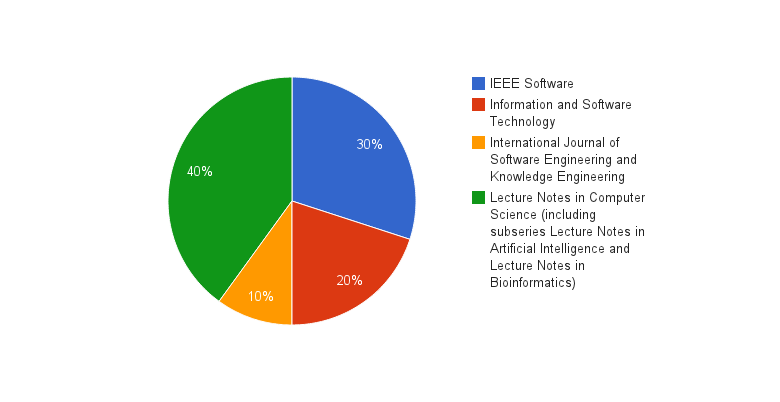
\includegraphics[width=200mm]{artikkelien_lehdet.png}
\caption{Lehdet, joissa valitut artikkelit on julkaistu.}
\label{artikkeli_lehdet_pie}
\end{figure}

\begin{center}
\begin{longtable}{|p{3cm}|p{4cm}|p{4cm}|p{4cm}|}
\caption{Artikkelien sisältämien retrospektiivimenetelmien vaiheet}\label{retrovaiheet_taulukko}\\ \hline
  & \textbf{Syötteen kehittäminen} & \textbf{Kausaalianalyysi} & \textbf{Parannusideoiden kehittäminen} \\
\hline
\endfirsthead
\multicolumn{4}{c}%
{\tablename\ \thetable\ -- \textit{Jatkoa edelliseltä sivulta}} \\
\hline
  & \textbf{Syötteen kehittäminen} & \textbf{Kausaalianalyysi} & \textbf{Parannusideoiden kehittäminen} \\
\hline
\endhead
\hline \multicolumn{4}{r}{\textit{Jatkuu seuraavalla sivulla}} \\
\endfoot
\hline
\endlastfoot
	\textbf{\citep{kalinowski2012evidence}} & 1) Ennen tapaamista kerätään sopiva datajoukko 2) Luokitellaan data 3) Pareto-chart:it mainitaan hyvänä tapana datan pääluokkien tunnistamiseen & Syy-seuraus-diagrammin, tarkemmin Fishbonen, piirtäminen mainitaan hyväksi todetuksi tavaksi tunnistaa systemaattisten ongelmien syitä. & - \\ \hline
	\textbf{\citep{Lehtinen2011}} & Fokus-ryhmän tapaaminen & 1) Kerätään syitä anonyymisti sähköpostitse. 2) Muodostetaan kerätyistä syistä suunntattu verkko 3) Brainwriting, brainstorming kokouksessa. Muodostetaan suunnattu verkko. 4) Tunnistetaan juurisyyt säköpostikyselyn avulla & Workshop, jossa parannusideoita kerätään brainwritingia yhdistettynä skeptiseen ja optimistiseen perspektiiviin. \\ \hline
	\textbf{\citep{Bjornson2009} menetelmä 1} & KJ-sessio & Fishbone (ryhmäkeskustelu) & - \\ \hline
	\textbf{\citep{Bjornson2009} menetelmä 2} & KJ-sessio & Kausaalikartan muodostaminen KJ-sessiossa & - \\ \hline
	\textbf{\citep{karlsson2006case}} & 1) Kerätään sopiva datajoukko (valitulle ohjelmistojulkaisulle toteutettuja vaatimuksia) 2) Uudelleenarvioidaan datajoukko 3) Visualisoidaan saatu data & 1) Keskustellaan visualisoidussa datassa ilmenevien ongelmien syistä. Fasilitaattori kirjoittaa keskustelusta muistiinpanoja. 2) Muistiinpanojen pohjalta luodaan taulukko, jolla löydetään eri datapisteille yhteisiä kategorioita (juurisyitä). & Kehitysideoiden kerääminen ja priorisointi \\ \hline
	\textbf{\citep{de2004learning}} & 1) Osallistujat täyttävät etukäteen kyselyn, joka toimii joko muistin virkistyksenä tai retrospektiivin fokuksen löytämisessä 2) KJ-sessio / Strukturoitu haastattelu & Fishbone (ryhmäkeskustelu) & - \\ \hline
	\textbf{\citep{staalhane2004root}} & Tehdään Pareto-analyysi defekteistä & 1) Fishbone (ryhmäkeskustelu) 2) Pisteytyksen avulla tunnistetaan olennaisimmat syyt (juurisyyt) & 1) Valituille syille brainstormataan kehitysideoita, jotka kootaan taulukkoon. Näistä äänestetään olennaisimmat, eli ne, jotka voitaisiin ottaa työn alle. \\ \hline
	\textbf{\citep{staalhane2003post} menetelmä 1} & 1) Fasilitaattori kerää etukäteen projektipäälliköltä taustatietoa projektista 2) KJ-sessio 3) KJ-session tulosten priorisointi & Fishbone & - \\ \hline
	\textbf{\citep{staalhane2003post} menetelmä 2} & 1) Fasilitaattori kerää etukäteen dokumenteista projektin taustatietoja 2) Strukturoitu haastattelu (valkotaulu ja fläppitaulu dokumentointina ja muistin tukena keskustelun ajan) & Syy-seuraus-suhteita tunnistetaan haastattelun aikana (fasilitaattorilla vastuu) & - \\ \hline
	\textbf{\citep{dingsoyr2003extending}} & KJ-sessio & Fishbone &  \\ \hline
	\textbf{\citep{birk2002postmortem}} & 1) Fasilitaattori tutustuu projektiin, käy mm. kaikki dokumentit läpi. 2) Asetetaan retrospektiiville tavoite 3) Kerätään positiivisia ja negatiivisia kokemuksia KJ-sessioilla,  semistrukturoiduilla haastatteluilla tai fasilitoiduilla ryhmäkeskusteluilla. & Fishbone (ryhmäkeskustelu) & - \\ \hline
	\textbf{\citep{card1998learning}} & 1) Valitaan sopiva datajoukko (voidaan tehdä etukäteen) 2) Luokitellaan datajoukko (voidaan tehdä etukäteen) 3) Tunnistetaan olennaisimmat datapisteet Parerto-chart:in avulla & Selvitetään ongelmien juurisyitä keskustelemalla ja tutkitaan löytyykö useammalla ongelmalla samoja syitä. Jos ongelman juurisyy ei löydy triviaalisti, käytetään Fishbone:a (ryhmäkeskusteluineen) apuna. & Fasilitoidun ryhmäkeskustelun avulla löydetään konkreettisia kehitysideoita. Näistä keskitytään niihin, joilla todennäköisimmiin on merkittävä vaikutus ongelmiin. \\ \hline
\end{longtable}
\end{center}


\section{Pohdinta}
\subsection{Retrospektiivien vaiheet}
Taulukossa \ref{retrovaiheet_taulukko} on kuvattu systemaattisessa kirjallisuuskatsauksessa löydetyt retrospektiivimenetelmät, jotka sisältävät juurisyyanalyysin yhtenä osana menetelmää.
Menetelmät voidaan jakaa kolmeen vaiheeseen: Syötteen kehittämiseen, kausaalianalyysiin ja parannusideoiden kehittämiseen. Jako on samankaltainen, kuin mitä Lehtinen on käyttänyt artikkelissaan \citep{Lehtinen2011}.

Artikkeleissa kuvatuissa menetelmissä kahdeksan kymmenestä suosittelee kausaalianalyysiin Ishikawa diagrammia (tunnetaan myös fishbone diagrammina) \citep{kalinowski2012evidence}, \citep{de2004learning}, \citep{staalhane2004root}, \citep{dingsoyr2003extending}, \citep{birk2002postmortem}, \citep{card1998learning}. Kahdella artikkelilla fishbone diagrammi oli kuvattu toisena menetelmänä jonkin muun rinnalla \citep{Bjornson2009}, \citep{staalhane2003post}.


kamaa johdannosta, sopiiko tänne?\\
\textit{Kandidaatintyössä tehdään synteesi kirjallisuuskatsauksessa kerätyssä aineistossa esitetyistä retrospektiivien juurisyyanalyysi-menetelmistä. On mahdollista, että osa aineistosta käsittelee raskaampaa, suuremman mittakaavan retrospektiiviä, joka pidettäisiin esimerkiksi projektin jälkeieen (post project review). Mikäli synteesin kuvaama menetelmä osoittautuu ketterän ohjelmistokehitystiimin retrospektiiviin liian raskaaksi, karsitaan siitä tähän tarkoitukseen ylimitoitetut kohdat pois. Lopputuloksen tulisi olla sellainen, että tiimi voi suorittaa sen ketterälle retrospektiiville varatussa, verrattain lyhyessä ajassa.}



\subsection{Kandidaatintyön validiteetti ja sen uhkat}
Systemaattisen kirjallisuuskatsauksen validiteettiin vaikuttaa luonnollisesti se, että sen on suurimmalta osin suorittanut yksi henkilö (kandidaatintyön kirjoittaja) oman arviokykynsä mukaan. Kandidaatityön ohjaaja on auttanut kandidaatintyön tekijää esimerkiksi hakusanojen valinnassa, mutta suorittava työ, kuten artikkeline arviointi ja rajaus on ollut kandidaatintyön tekijän vastuulla. On mahdollista, että joitain olennaisia artikkeleja karsiutui väärin perustein pois, koska abstraktia oli tulkittiin väärin. On myös todennäköistä, ettei valittuhakutermimme saavuttanut kaikkia olennaisia artikkeleja, mikäli ne eivät sisältäneet käytettyjä hakusanoja.

Silti on perusteltua pitää suoritettua systemaattista kirjallisuuskatsausta huomattavasti luotettavampana ja tieteellisempänä tutkimusmenetelmänä, kuin tyypillinen sattumanvaraisten, erilaisten hakusanojen kokeilu eri hakukoneissa ja niiden hakutuloksista mielivaltaisin perustein valittujen artikkelien lukeminen. Tarkat ja hyvin dokumentoidut artikkelien valintakriteerit ja muut systemaattisen kirjallisuuskatsauksen eri vaiheet tekevät tutkimuksesta helposti toistettavan ja tarkistettavan. Tämä parantaa tehdyn tutkimuksen validiteettia huomattavsti.

Lisäksi aineistohaun rajaaminen ennalta karsittuun joukkoon (Scopus-hakukone) ja sieltä pelkkien tieteellisten artikkelien, jotka käyvät julkaisuvaiheessa tiukan karsintaprosessin, valinta parantaa käsitellyn aineiston luotettavuutta.

\section{Yhteenveto}
